\documentclass{beamer}
%
% Choose how your presentation looks.
%
% For more themes, color themes and font themes, see:
% http://deic.uab.es/~iblanes/beamer_gallery/index_by_theme.html
%
\usetheme{Madrid}
%\mode<presentation>
%{
%  \usetheme{Boadilla}     % or try Boadilla, Darmstadt, Madrid, Warsaw, default, ...
%  \usecolortheme{default} % or try Boadilla, albatross, beaver, crane, default, ...
%  \usefonttheme{default}  % or try Boadilla, serif, structurebold, default, ...
%  \setbeamertemplate{navigation symbols}{}
%  \setbeamertemplate{caption}[numbered]
%} 

\usepackage{listings}

\usepackage{tikz}

\usepackage{movie15}
\usepackage{media9}

\usepackage{color}

 \usepackage{multirow}
 \usepackage[font=scriptsize]{caption}
 \usepackage{cite}
\usepackage{graphicx}
\usepackage{amsmath}
\usepackage{tikz}
\usepackage[font = small]{caption}

\usepackage[english]{babel}
\usepackage[utf8x]{inputenc}
\usepackage{color}


\AtBeginSubsection[]
{
  \begin{frame}<beamer>{Outline}
    \tableofcontents[currentsection,currentsubsection]
  \end{frame}
}


\begin{document}

\begin{frame}

\title[Module 1]{Data communication using single board computers}
\subtitle{}
\author[Prakruti Mallayya Bilagi] {A breif Review of the program}

\institute[]{{Presented by : Prakruti M Bilagi\\2014IEN36\\Central university of Karnataka}}
\date{Guide : Dr. G V V Sharma\\Dept of EE\\Indian Institute of Technology Huderabad}
\maketitle
    
\end{frame}







\begin{frame}{The code package}
\bullet \qquad  Pcm\_wave\_header.h\\
\bullet \qquad  Audioformat.h \\
\bullet \qquad  Error\_reporter.h\\
\bullet \qquad  Error\_reporter.cpp\\ 
\bullet \qquad  Main.cpp \\
\bullet \qquad  Transmitter.h  \\
\bullet \qquad  Transmitter.cpp \\
\bullet \qquad  Wave\_reader.h\\
\bullet \qquad  Wave\_reader.cpp\\
\bullet \qquad  Makefile \\
\bullet \qquad  Acaustic\_guiter.wav \\



\end{frame}




\begin{frame}{Pcm\_wave\_header }
\begin{minipage}{0.6 \textwidth}
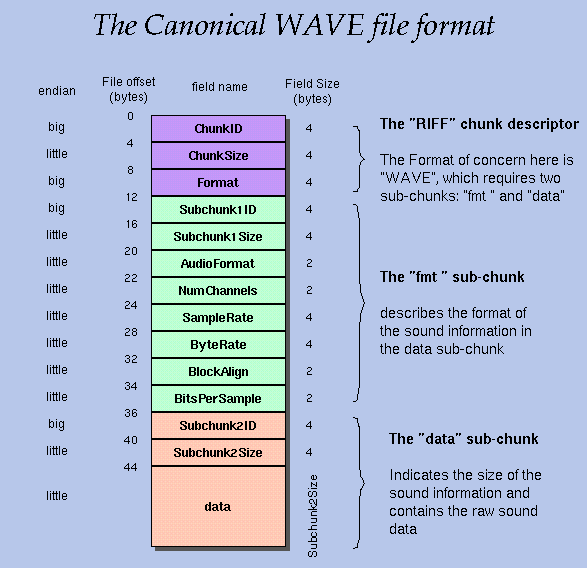
\includegraphics[scale=0.3]{wave.png}
\end{minipage}
\begin{minipage}{0.38 \textwidth}
struct PCMWaveHeader\\
\{\\
    char chunkID[4];\\
    unsigned chunkSize;\\
    char format[4];\\
    char subchunk1ID[4];\\
    unsigned subchunk1Size;\\
    unsigned short audioFormat;\\
    unsigned short channels;\\
    unsigned sampleRate;\\
    unsigned byteRate;\\
    unsigned short blockAlign;\\
    unsigned short bitsPerSample;\\
    char subchunk2ID[4];\\
    unsigned subchunk2Size;\\
\};\\

\end{minipage}

\end{frame}




\begin{frame}{Audioformat.h}
struct AudioFormat\\
\{\\
 \qquad   unsigned short channels;\\
   \qquad  unsigned short bitsPerSample;\\
    \qquad unsigned sampleRate;\\
\};\\
\end{frame}

\begin{frame}{ErrorReporter.h}
using std::exception;\\
using std::string;\\

class ErrorReporter : public exception\\
\{ \\
   \qquad  public:\\
   \qquad \qquad     explicit ErrorReporter(string message);\\
   \qquad \qquad   virtual ~ErrorReporter() throw();        \\

   \qquad \qquad	virtual const char* what() const throw();\\
   \qquad protected:\\
    \qquad\qquad  string errorMessage;\\
\}; \\

\end{frame}




\begin{frame}{ErrorReporter.cpp}

\#include "error\_reporter.h"\\

ErrorReporter::ErrorReporter(string message) :\\
   \qquad errorMessage(message) \\
\{ \\
\} \\

ErrorReporter::~ErrorReporter() throw() \\
\{ \\
\} \\
		
const char* ErrorReporter::what() const throw()\\
\{ \\
\qquad	return errorMessage.c\_str();\\
\} \\


\end{frame}


\begin{frame}{Main.cpp}
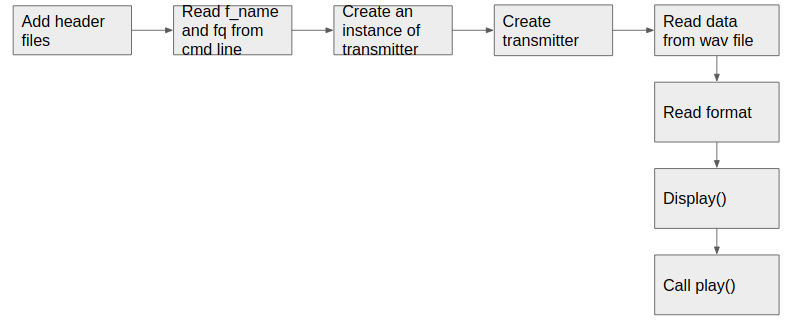
\includegraphics[scale=0.4]{maiin.png}

\end{frame}



\begin{frame}{Tranmitter.h}
class Transmitter\\
\{\\
\qquad  public:\\
    \qquad \qquad    virtual  Transmitter();\\

      \qquad \qquad  void play(string filename, double frequency, bool loop);\\
       \qquad \qquad void stop();

      \qquad \qquad  static Transmitter* getInstance();\\
\qquad private:\\
       \qquad \qquad Transmitter();\\

       \qquad \qquad bool forceStop, eof;\\

       \qquad \qquad static void* peripherals;\\
        \qquad \qquad static vectorfloat* buffer;\\
       \qquad \qquad static bool transmitting, restart;\\
       \qquad \qquad static unsigned frameOffset, clockDivisor;\\
       \qquad \qquad static void* transmit(void* params);\\
\};\\

\end{frame}




\begin{frame}{Transmitte.cpp}
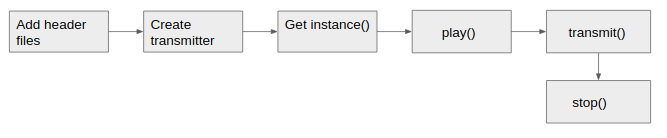
\includegraphics[scale=0.5]{tran.png}
\begin{itemize}
\item  Include header files \\

\item Assign the base addresses for gpio base clock base clockdividor base and a counter \\

\item Assign initial values for variables to transmitter class members
\item Check for the system, type and version  of the host system.

\item Assign memory for the GPIO pins using memFd and mmap system calls and this memory would be the base for assessing the GPIO and clock etc. 




\end{itemize}
 

\end{frame}





\begin{frame}{Transmitter conti\...}
\begin{itemize}
\item In the function play()
\item[a] It checks if the transmitter is already transmitting something. 
\item[b] Creates the objects of class Wave\_reader.(reader)
\item[c] Grab the format of the reader and store it in "format" variable.
\item[d] Set the value to the clockDivisor.
\item[e] Create the bufferFrames that will be stored in the vector "frames"
\item[f] Create a vector "Frames" and use the fuction getFrames from class reader to stack the bufferFrames into it.
 
\item[g] Create thread to start the transmission.

\item[h] Read the whole data frames one by one. 
\item[i] Set "transmitting" variable "false".
\item[j] Join the thread.
\item[k] Delete the reader and format finally while exiting.
\end{itemize}

\end{frame}

\begin{frame}{Transmitter conti\...}
\begin{itemize}
\item Next comes the transmit() function where in does the changes in the clock frequency for the transmission purpose.
\item [a] Declares variables to store the current, start and playbackstart positions of the data.
\item[b] Creates unsigned offset, length and temp variables.
\item[c] Creates a vectr of floats to hold the data.
\item[d] Loads the sample-rate into a variable.
\item[e] Assigns the preemp value of 0.734883 $ preemp=\frac{0.75-2500000.0}{(float)(samplerate*75)} $
\item[f] Sets the GPIO pin 4 on alternate function-0.
\item[h] Enables the clock-base pin.
\item[i] The playback starts
\item[j] Assigning of value and quantize it between -1, value, 1
\item[k] Set the clockdividor base register.
\item[l] Increment the counter register.
\item[m] Disable the clock base pin.
\item When the interrupt is generated from the keyboard the the transmission/FM is aborted.
\end{itemize}
\end{frame}
\begin{frame}{Wave\_reader.h}
class WaveReader\\
\{\\
   \qquad public:\\
    \qquad  \qquad     WaveReader(string filename, bool &forceStop);\\
        \qquad  \qquad virtual ~WaveReader();\\

     \qquad  \qquad    AudioFormat* getFormat();\\
 \qquad  \qquad     vector<float>* getFrames(unsigned frameCount, bool &forceStop);\\
     \qquad  \qquad  bool setFrameOffset(unsigned frameOffset);\\
     \qquad   private:\\
       \qquad \qquad  string filename;\\
       \qquad \qquad  PCMWaveHeader header;\\
       \qquad \qquad  unsigned dataOffset, currentOffset;\\
        \qquad \qquad int fileDescriptor;\\

       \qquad \qquad  vector\<char\>* readData(unsigned bytesToRead, bool\\ \qquad \qquad  headerBytes, bool &forceStop);\\
      \qquad \qquad   string getFilename();\\
\};\\


\end{frame}

\begin{frame}{Wave\_reader.cpp}
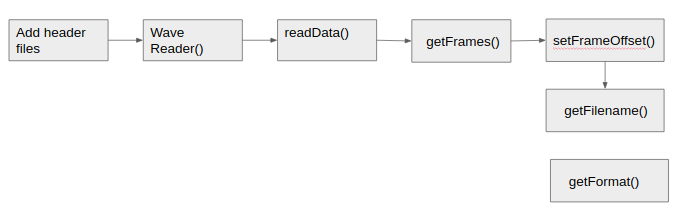
\includegraphics[scale=0.5]{wavereaer.png}

\begin{itemize}
\item Includes header files.
\item It has a function for WaveReader(), which will read the entire data in the wavefile.
\item It has a dataread() which will read the specified bytes from the file and returns the data vector.
\item It has a getFrames() function that will read the perticular count of frames and return the vector frame.
\item Setframeoffset() function will create the shift in the data frames.

\item getfilename() is a function that will return the file name of the WAV file

\item Getformat() is a function that will return the information about the channels, sample rate, bitspersample. 




\end{itemize}


\end{frame}



\begin{frame}{Makefile}
As the name suggests it is make file which allows for the execution on this FM on particular processor

\end{frame}

\end{document}